\documentclass[a4paper, 12pt, french]{article}
\usepackage[utf8]{inputenc}
\usepackage[T1]{fontenc}
\usepackage{babel}
\usepackage{setspace}
\usepackage{hyperref}
\usepackage{imakeidx}
\usepackage{graphicx}
\usepackage{fancyhdr}
\usepackage{chngcntr}
\usepackage{pifont}
\usepackage{xcolor}
\usepackage{glossaries}
\usepackage{helvet}
\usepackage{titlesec}
\usepackage{tikz}
\usepackage{rotating}
\usepackage{lscape}
\usepackage{wrapfig}
\usepackage[stable]{footmisc}

\makeindex[intoc]
 
\counterwithin{figure}{section}
\counterwithin{table}{section}

\definecolor{ssiYellow}{RGB}{255,237,0}
\definecolor{ssiRed}{RGB}{231,0,14}
\definecolor{ssiBlack}{RGB}{18,18,13}

\newcommand{\bdot}{\item[\color{ssiYellow}\ding{108}]} 
\newcommand{\bdotoutlined}{\item[\color{ssiYellow}\ding{109}]}
\newcommand{\bsquare}{\item[\color{ssiYellow}\ding{110}]} 

\hypersetup{%
    pdfborder = {0 0 0}
}
\renewcommand{\familydefault}{\sfdefault}

\titleformat{name=\section}{\normalfont\Large\bfseries\color{ssiBlack}}{\color{ssiYellow}\rule[-1.35mm]{3em}{1.25em}{\color{white}\hspace{-1cm}\normalfont\Large\bfseries\thesection\hspace{15pt}}}{1em}{}[\color{ssiYellow}{\titlerule[4pt]}\vspace*{4pt}]
\titleformat{\subsection}{\normalfont\Large\bfseries\color{ssiBlack}}{\color{ssiRed}\rule[-1.35mm]{3em}{1.25em}{\color{white}\hspace{-1.3cm}\normalfont\Large\bfseries\thesubsection\hspace{10pt}}}{1em}{}[\color{ssiYellow}{\titlerule[3pt]}\vspace*{4pt}]
\titleformat{\subsubsection}{\normalfont\Large\bfseries\color{ssiBlack}}{\color{ssiYellow}\rule[-1.35mm]{3em}{1.25em}{\color{white}\hspace{-1.60cm}\normalfont\Large\bfseries\thesubsubsection\hspace{5pt}}}{1em}{}[\color{ssiYellow}{\titlerule[2pt]}\vspace*{4pt}]

\titleformat{name=\section,numberless=true}{\color{ssiBlack}\normalfont\Large\bfseries}{}{0em}{}[\color{ssiYellow}{\titlerule[4pt]}\vspace*{4pt}]
\titleformat{name=\subsection,numberless=true}{\color{ssiBlack}\normalfont\Large\bfseries}{}{0em}{}[\color{ssiYellow}{\titlerule[3pt]}\vspace*{4pt}]
\titleformat{name=\subsubsection,numberless=true}{\color{ssiBlack}\normalfont\Large\bfseries}{}{0em}{}[\color{ssiYellow}{\titlerule[2pt]}\vspace*{4pt}]

\sloppy

\pagestyle{fancy}
\fancyhf{}
\rhead{Informatique et réseaux}
\lhead{PINEAU Anthony}

\begin{document}
	\begin{titlepage}
		\begin{center}

			\tikz[remember picture,overlay] \node[opacity=0.3,inner sep=0pt] at (current page.center){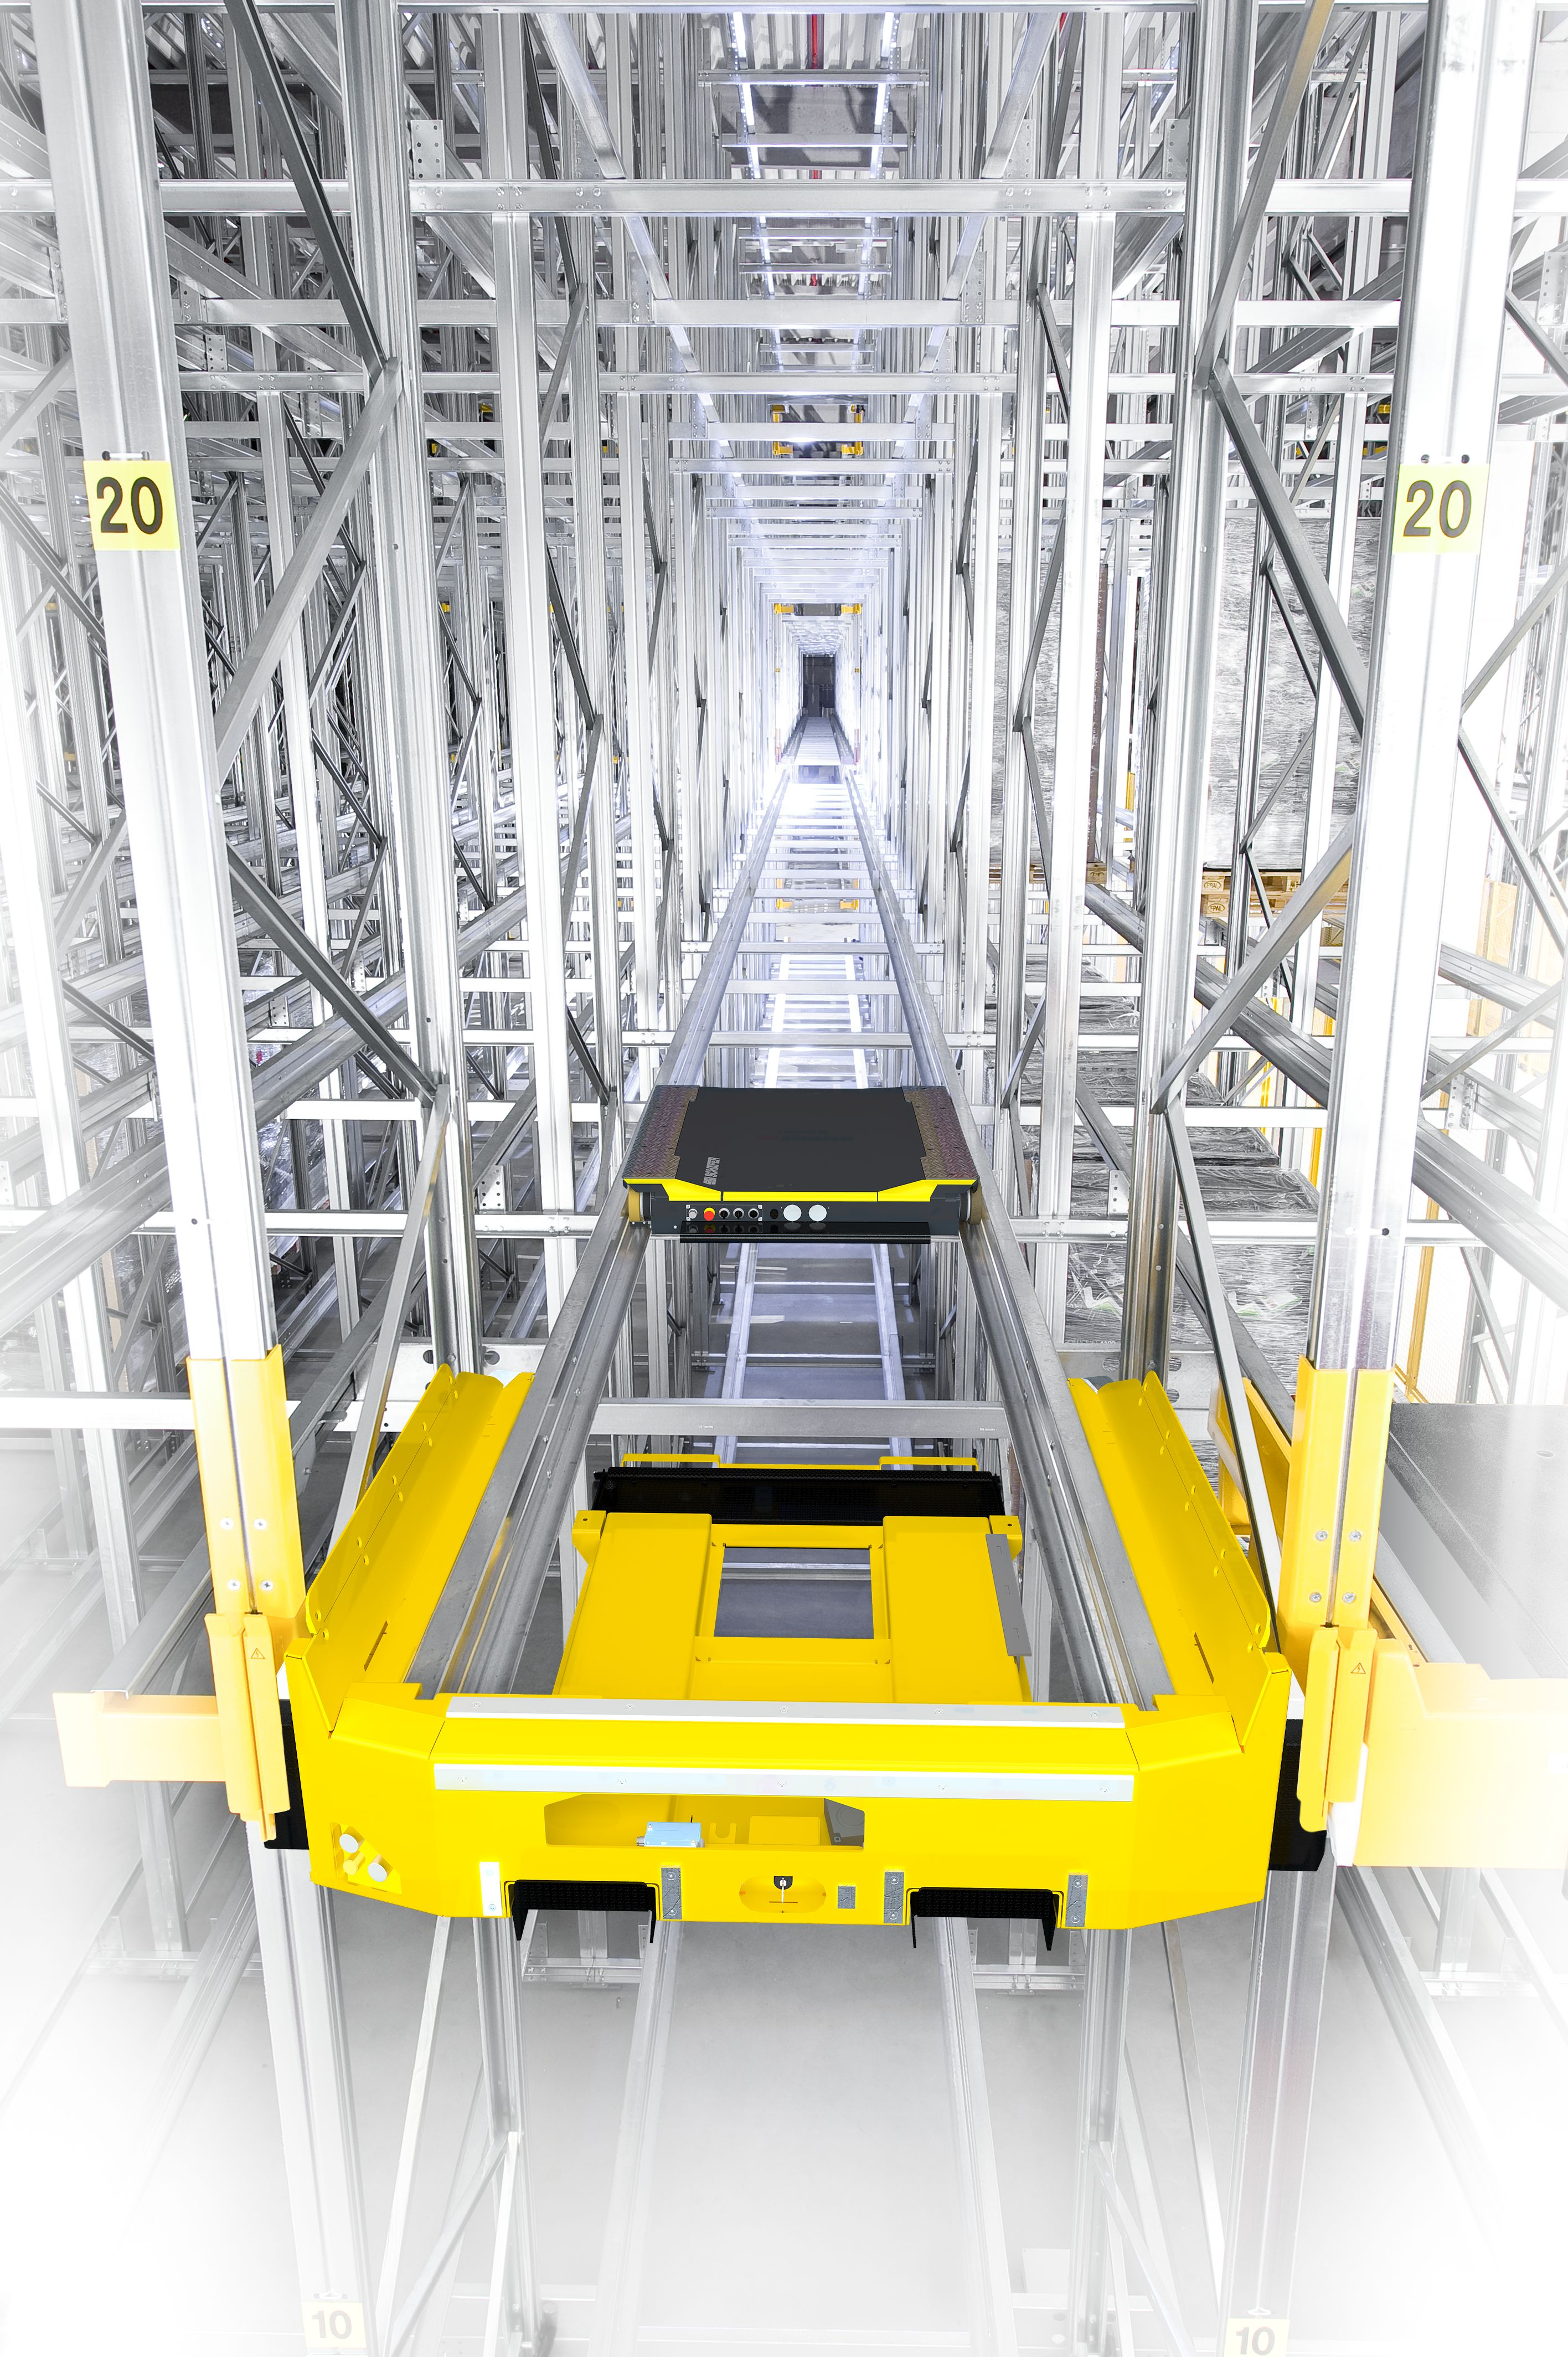
\includegraphics[width=\paperwidth,height=\paperheight]{../images/ssi_orbiter_highlight.jpg}};

			%\vspace*{1cm}

			\Huge
			\textbf{Rapport d'avancement}

			\vspace{0.5cm}
			\LARGE
			"Client Morpheus WEB"

			\vspace{1.5cm}

			\textbf{Anthony PINEAU}\\
			\textbf{IR2023}

			\vfill

			
\includegraphics[width=0.6\textwidth]{../images/schaefer.jpg}
			\vfill
			
\includegraphics[width=0.4\textwidth]{../images/esaip.jpg}

			\vfill

			Période effectuée du\\
			13 mars 2023 au 14 avril 2023

			\vspace{0.8cm}
			
			\Large
			Maître de stage : Monsieur Thierry NEROT\\
			Tuteur pédagogique : Monsieur Sofiane HAMRIOUI\\
		\end{center}
	\end{titlepage}
		
	\newpage
	
	\doublespacing
	\tableofcontents

	\newpage
		
	\rfoot{Page \thepage}
	
%	\phantomsection
%	\listoffigures
%	\addcontentsline{toc}{section}{\listfigurename}
	
%	\newpage
	
	\singlespacing

	\phantomsection
	\section{Sujet}
		Le lancement du projet a pour origine la volonté de développer un nouveau client Morpheus avec un nouveau design et compatible avec les technologies web.\\

		\noindent Les limites du projet sont :

		\begin{itemize}
			\bdot{Etude des composants TMS pour le développement en Delphi X10, 2 pages HTML5}
			\bdot{Construction d’un nouveau projet d’un nouveau client Morpheus}
			\bdot{Définition d’une nouvelle interface graphique}
			\bdot{Etude d’un mode de paramétrage graphique par l’utilisateur final}
			\bdot{Développement d’une maquette}
			\bdot{Développement de la technologie HTML 5 sous Delphi X10 en Pascal et génération et lecture fichier XML}
			\bdot{Intégration d’un serveur rest pilotant en JSON}
		\end{itemize}
		\vspace{\baselineskip}
		\par Les utilisateurs finaux sont les utilisateurs de morpheus. Ce sont donc ainsi des techniciens logistiques qui travaillent dans des entrepôts

	\newpage

	\section{Objectifs de la structure d'acceuil par rapport au projet}
		\noindent Les objectifs du projet sont :
		\begin{itemize}
			\bdot{Développer un client morpheus full html 5 responsive pour une partie des fenêtres du client morpheus existant}
			\bdot{Expérimenter les outils de développement tms web}
			\bdot{Faire une maquette d'interface utilisateur}
				\begin{itemize}
					\bdotoutlined{Fenêtre main (principale)}
						\begin{itemize}
							\bsquare{Menu}
							\bsquare{Boutons de fonction}
							\bsquare{Treeview}
						\end{itemize}
					\bdotoutlined{Login}
					\bdotoutlined{Connexion à la base de données}
					\bdotoutlined{Gestion des styles}
					\bdotoutlined{Gestion multi-fenêtres mdi}
				\end{itemize}
			\bdot{Rédiger un descriptif du mode de fonctionnement du client au niveau ergonomique}
			\bdot{Développer une première version avec les fenêtres de base}
				\begin{itemize}
					\bdotoutlined{Fenêtre main (principale)}
						\begin{itemize}
							\bsquare{Menu}
								\begin{itemize}
									\bdot{Icones}
									\bdot{Style ( comme style windows : couleurs)}
									\bdot{X niveaux et sous niveaux paramètrables : par rapport à une bdd afficher ou pas des points d'entrées du menu}
								\end{itemize}
							\bsquare{Boutons de fonction}
								\begin{itemize}
									\bdot{Style}
									\bdot{Icones}
									\bdot{Taille des boutons (16, 32 ou 48)}
									\bdot{Rendre visible ou non les boutons}
									\bdot{Mise en page des boutons en fonction du nombre : alignements...}									
								\end{itemize}
							\bsquare{Treeview}
								\begin{itemize}
									\bdot{Style}
									\bdot{Icones (devant nom sans toucher au petit triangle)}
									\bdot{Afficher une liste sur un niveau suivant une requête}
									\bdot{Charger les arborescences dynamiques (si on clique sur site afficher les sites et pas avant) : paramétrage visible ou non des arborescences}
								\end{itemize}
						\end{itemize}
					
					\bdotoutlined{Gestion des styles}
					\bdotoutlined{Gestion multi-fenêtres mdi (tabs)}
						\begin{itemize}
							\bsquare{Icones}
							\bsquare{Fermable ou non par une croix}
						\end{itemize}
					\bdotoutlined{Gestion fenêtres modales (gestion croix ou non et mémorisation de position)}
					\bdotoutlined{Login}
					\bdotoutlined{Connexion à la base de données}
					\bdotoutlined{Gestion des droits d'accès}
					\bdotoutlined{Gestion paramétrage en xml des fenêtres}
						\begin{itemize}
							\bsquare{Type de fenêtre}
							\bsquare{Grid associé}
							\bsquare{Requête sql}
						\end{itemize}
				\end{itemize}
		\end{itemize}

	\newpage

	\section{Moyens mis à disposition}
	\noindent Les moyens mis à ma disposition sont :
	\begin{itemize}
			\bdot{un ordinateur portable avec station d'accueil}
			\bdot{deux écrans}
			\bdot{environnement de développement intégré delphi 11.3}
			\bdot{composants tms software}
			\bdot{suite microsoft office : word, outlook, teams...}
	\end{itemize}	
	
	\section{Position du stagiaire dans le projet}
		Ma position au sein du projet est développeur de l'application web.

	\section{Enjeux pour la structure d'accueil}
		L'enjeu du projet pour la structure d'accueil est le développement d’un nouveau client Morpheus avec un nouveau design et compatible avec les technologies web.

	\section{Éventuelles modifications de la mission de l'élève ingénieur par rapport à la description réalisée}
   		Aucune modification de la mission par rapport à la description réalisée pour le moment.
		
\end{document}